%%%%%%%%%%%%%%%%%%%%%%%%%%%%%%%%%%%%%%%%%
% http://www.LaTeXTemplates.com
% License:
% CC BY-NC-SA 3.0 (http://creativecommons.org/licenses/by-nc-sa/3.0/)
%%%%%%%%%%%%%%%%%%%%%%%%%%%%%%%%%%%%%%%%%


\documentclass{beamer}

\mode<presentation> {
	\usetheme{Madrid}
}

\usepackage{graphicx} % Allows including images
\usepackage{booktabs} % Allows the use of \toprule, \midrule and \bottomrule in tables
\usepackage{pdfpages}
\usepackage[percent]{overpic}

\usepackage{tikz}
\usetikzlibrary{calc,trees,positioning,arrows,chains,shapes.geometric,%
	decorations.pathreplacing,decorations.pathmorphing,shapes,%
	matrix,shapes.symbols}

\tikzset{
	>=stealth',
	punktchain/.style={
		rectangle, 
		rounded corners, 
		% fill=black!10,
		draw=black, very thick,
		text width=10em, 
		minimum height=3em, 
		text centered, 
		on chain},
	line/.style={draw, thick, <-},
	element/.style={
		tape,
		top color=white,
		bottom color=blue!50!black!60!,
		minimum width=8em,
		draw=blue!40!black!90, very thick,
		text width=10em, 
		minimum height=3.5em, 
		text centered, 
		on chain},
	every join/.style={->, thick,shorten >=1pt},
	decoration={brace},
	tuborg/.style={decorate},
	tubnode/.style={midway, right=2pt},
}

\newcommand*\circled[1]{\tikz[baseline=(char.base)]{
		\node[shape=circle,draw,inner sep=2pt] (char) {#1};}}

%----------------------------------------------------------------------------------------
%   TITLE PAGE
%----------------------------------------------------------------------------------------

\title[FlashTalk 1]{FlashTalk 1:  Enumerating the inorganic universe of small complexes for machine learning} % The short title appears at the bottom of every slide, the full title is only on the title page

\author{Stefan Gugler} % Your name
\institute[MIT] % Your institution as it will appear on the bottom of every slide, may be shorthand to save space
{
	Massachusetts Institute of Technology \\ % Your institution for the title page
	\medskip
	\textit{sgugler@mit.edu} % Your email address
}
\date{\today} % Date, can be changed to a custom date

\begin{document}
	
\begin{frame}
	\titlepage % Print the title page as the first slide
\end{frame}

%\begin{frame}
%\frametitle{Overview} % Table of contents slide, comment this block out to remove it
%\tableofcontents % Throughout your presentation, if you choose to use \section{} and \subsection{} commands, these will automatically be printed on this slide as an overview of your presentation
%\end{frame}

%----------------------------------------------------------------------------------------
%   PRESENTATION SLIDES
%----------------------------------------------------------------------------------------

%------------------------------------------------
%\section{First Section} % Sections can be created in order to organize your presentation into discrete blocks, all sections and subsections are automatically printed in the table of contents as an overview of the talk
%------------------------------------------------

%\subsection{Subsection Example} % A subsection can be created just before a set of slides with a common theme to further break down your presentation into chunks

\begin{frame}
\frametitle{Reduction of the full small ligand universe: Mo, Di, Bi}

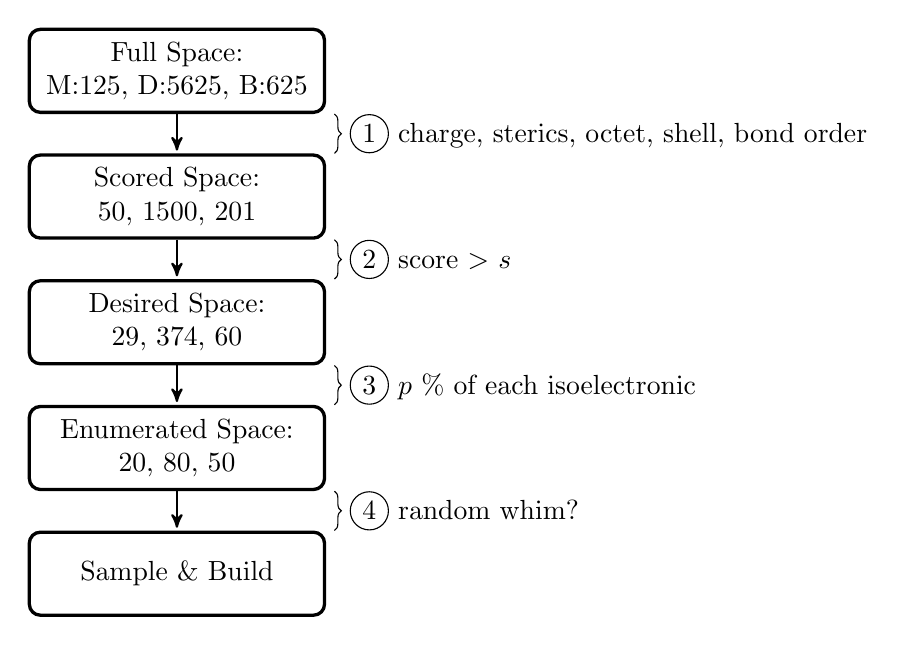
\begin{tikzpicture}
[node distance=.5cm,
start chain=going below,]
\node[punktchain, join] (full) {Full Space: \\ M:125, D:5625, B:625};
\node[punktchain, join] (scored){Scored Space: \\ 50, 1500, 201};
\node[punktchain, join] (desi){Desired Space: \\ 29, 374, 60};
\node[punktchain, join] (enum){Enumerated Space: \\ 20, 80, 50};
\node[punktchain, join] (sampl){Sample \& Build };

\draw[tuborg, decoration={brace}] let \p1=(full.south), \p2=(scored.north) in
($(2, \y1)$) -- ($(2, \y2)$) node[tubnode] {\circled{1} charge, sterics, octet, shell, bond order};
\draw[tuborg] let \p1=(scored.south), \p2=(desi.north) in
($(2, \y1)$) -- ($(2, \y2)$) node[tubnode] {\circled{2} score $>$ $s$};
\draw[tuborg] let \p1=(desi.south), \p2=(enum.north) in
($(2, \y1)$) -- ($(2, \y2)$) node[tubnode] {\circled{3} $p$ \% of each isoelectronic};
\draw[tuborg] let \p1=(enum.south), \p2=(sampl.north) in
($(2, \y1)$) -- ($(2, \y2)$) node[tubnode] {\circled{4} random whim?};
\end{tikzpicture}


\end{frame}


\begin{frame}
\frametitle{Distribution and Examples}
\centering
\begin{overpic}[width=0.8\linewidth]{img/distrDiCNOPS.pdf}
	\put (13,24) {[C--]=[OH2--]}
	\put (15,31) {[N--]-[PH4--]}
	\put (25,37) {[CH3]-[SH2-]}
	\put (30,45) {[PH++]\#0[SH3-]}
	
	\put (56,53) {[NH2]-[OH]}
	\put (80,57) {[C+]\#[O-]}
	\put (78,51) {[O-]\#[O-]}
\end{overpic}
\end{frame}



\end{document}